%%%%%%%%%%%%%%%%%%%%%%%%%%%%%%%%%%%%%%%%%
% Beamer Presentation
% LaTeX Template
% Version 1.0 (10/11/12)
%
% This template has been downloaded from:
% http://www.LaTeXTemplates.com
%
% License:
% CC BY-NC-SA 3.0 (http://creativecommons.org/licenses/by-nc-sa/3.0/)
%
%%%%%%%%%%%%%%%%%%%%%%%%%%%%%%%%%%%%%%%%%

%----------------------------------------------------------------------------------------
%	PACKAGES AND THEMES
%----------------------------------------------------------------------------------------

\documentclass[professionalfonts]{beamer}

\mode<presentation> {

% The Beamer class comes with a number of default slide themes
% which change the colors and layouts of slides. Below this is a list
% of all the themes, uncomment each in turn to see what they look like.

%\usetheme{default}
%\usetheme{AnnArbor}
%\usetheme{Antibes}
%\usetheme{Bergen}
%\usetheme{Berkeley}
%\usetheme{Berlin}
%\usetheme{Boadilla}
%\usetheme{CambridgeUS}
%\usetheme{Copenhagen}
%\usetheme{Darmstadt}
%\usetheme{Dresden}
%\usetheme{Frankfurt}
%\usetheme{Goettingen}
%\usetheme{Hannover}
%\usetheme{Ilmenau}
%\usetheme{JuanLesPins}
%\usetheme{Luebeck}
\usetheme{Madrid}
%\usetheme{Malmoe}
%\usetheme{Marburg}
%\usetheme{Montpellier}
%\usetheme{PaloAlto}
%\usetheme{Pittsburgh}
%\usetheme{Rochester}
%\usetheme{Singapore}
%\usetheme{Szeged}
%\usetheme{Warsaw}

% As well as themes, the Beamer class has a number of color themes
% for any slide theme. Uncomment each of these in turn to see how it
% changes the colors of your current slide theme.

%\usecolortheme{albatross}
%\usecolortheme{beaver}
%\usecolortheme{beetle}
%\usecolortheme{crane}
%\usecolortheme{dolphin}
%\usecolortheme{dove}
%\usecolortheme{fly}
%\usecolortheme{lily}
%\usecolortheme{orchid}
%\usecolortheme{rose}
%\usecolortheme{seagull}
%\usecolortheme{seahorse}
%\usecolortheme{whale}
%\usecolortheme{wolverine}

%\setbeamertemplate{footline} % To remove the footer line in all slides uncomment this line
%\setbeamertemplate{footline}[page number] % To replace the footer line in all slides with a simple slide count uncomment this line

%\setbeamertemplate{navigation symbols}{} % To remove the navigation symbols from the bottom of all slides uncomment this line
}
%\usepackage{CJK}
\usepackage{graphicx} % Allows including images
\usepackage{booktabs} % Allows the use of \toprule, \midrule and \bottomrule in tables
\usepackage{amsfonts}
\usepackage{color}


%----------------------------------------------------------------------------------------
%	TITLE PAGE
%----------------------------------------------------------------------------------------

\title[Complex Networks]{Complex Networks} % The short title appears at the bottom of every slide, the full title is only on the title page

\author{Chen SiYu} % Your name
\institute[ZJU] % Your institution as it will appear on the bottom of every slide, may be shorthand to save space
{
Zhejiang University \\ % Your institution for the title page
\medskip
\textit{sychen@zju.edu.cn} % Your email address
}
\date{\today} % Date, can be changed to a custom date
\begin{document}
\LARGE
\everymath{\displaystyle}


\begin{frame}
\titlepage % Print the title page as the first slide
\end{frame}

\begin{frame}
\frametitle{Overview} 
\tableofcontents
\end{frame}

%----------------------------------------------------------------------------------------
%	PRESENTATION SLIDES
%----------------------------------------------------------------------------------------


\section{Why Complex Networks?} 
%------------------------------------------------
\begin{frame}
\frametitle{Why Complex Networks?}
Concepts
\begin{itemize}
\item Community evolution
\item Overlapping communities
\item Directed networks
\item Community characterization\ interpretation
\item Modularities
\end{itemize}
\end{frame}


\begin{frame}
\frametitle{Why Complex Networks?}
\begin{itemize}
\item Unifying principles
\item Dynamics
\end{itemize}
\end{frame}

\begin{frame}
\frametitle{What for?}
\begin{itemize}
\item prevailing products 
\item key users @Tc
\item hot topics, ads
\item followings, sortings
\item clustering genes.
\end{itemize}
\end{frame}

\section{What is Complex Networks?}

\begin{frame}
\frametitle{Definition by QIAN XueSen}
\begin{itemize}
\item self-organizing
\item sefl-similar
\item attractor (simple,singular)
\item small-world
\item scale-free (power-law)
\end{itemize}
\end{frame}


\begin{frame}
\frametitle{self similar}
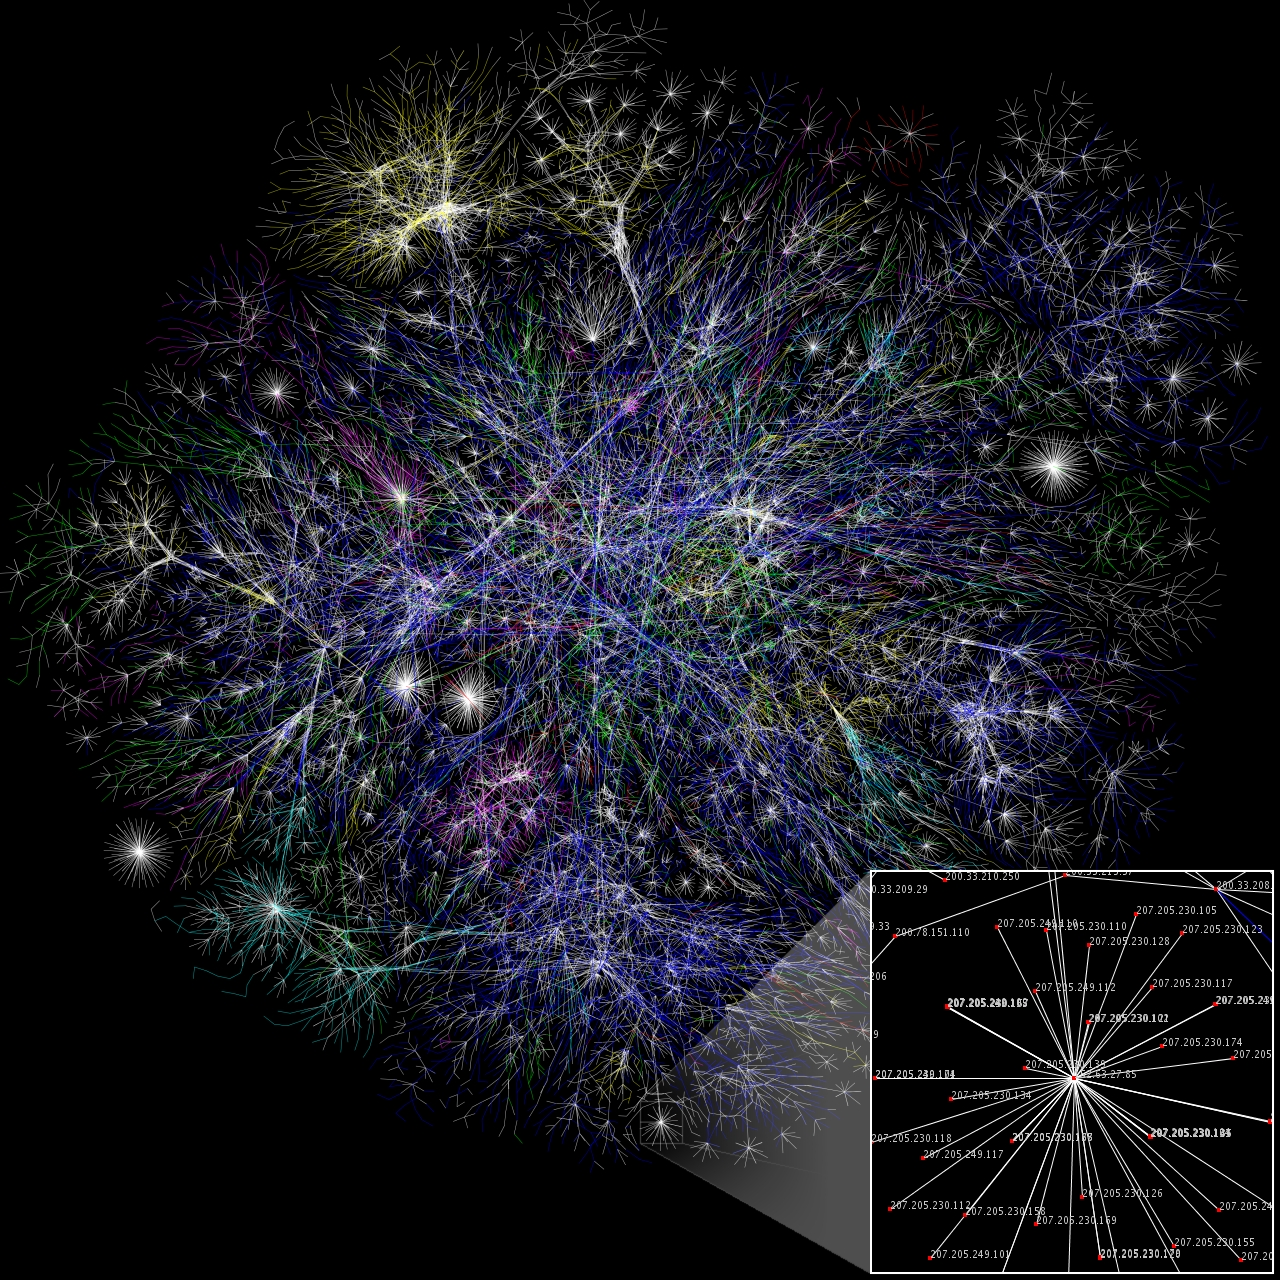
\includegraphics[height=9cm]{complexnet}
\end{frame}

\begin{frame}
\frametitle{power law (long tail)}
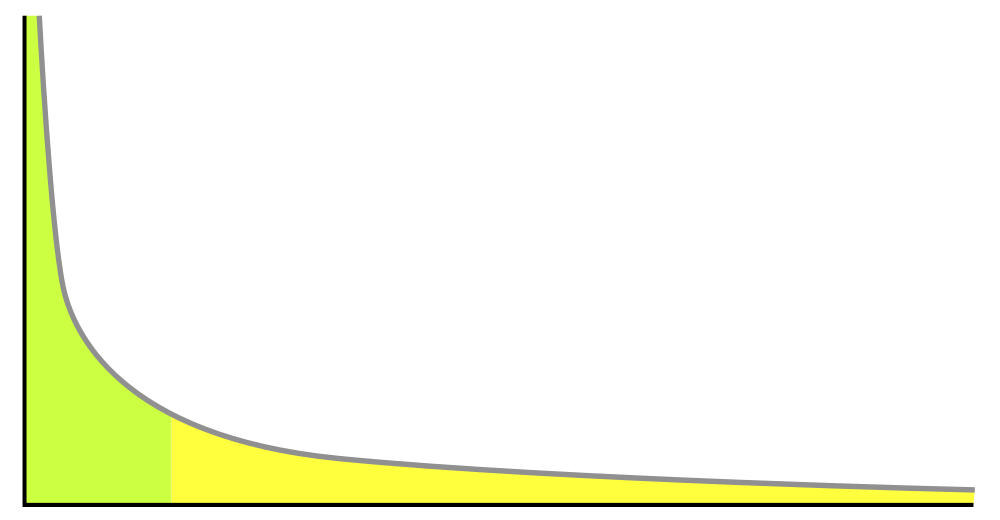
\includegraphics[height=5cm]{powerlaw}
\begin{itemize}
\item [X] frequency of words
\item [Y] priority when using
\end{itemize}(Degree,Closeness$\infty$,Harmonic Centrality)
\end{frame}


\begin{frame}
\frametitle{small world}
small world experiment by Milgram, 1967
\begin{columns}[c]
\column{.7\textwidth}
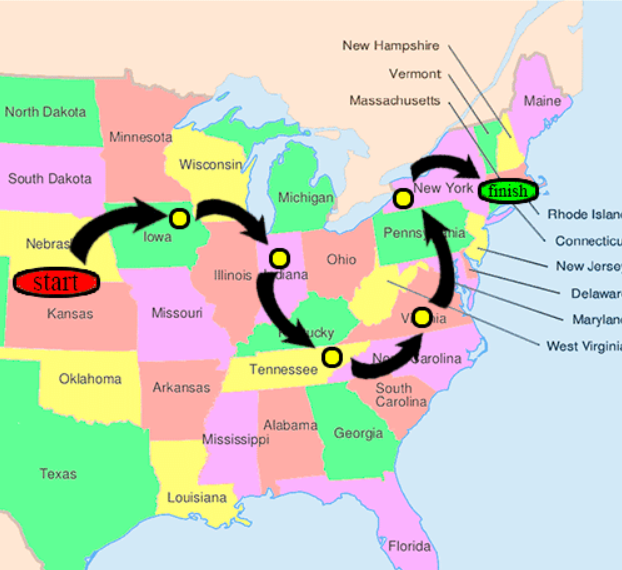
\includegraphics[height=7cm]{smallworld}

\column{.3\textwidth}
\begin{itemize}
\item 232/296
\item 64
\item 5.5-6
\end{itemize}
\end{columns}
\end{frame}

\begin{frame}
\frametitle{Characteristic}
\begin{itemize}
\item Assortative Mixing: 
$E(i,j), \Delta(node_i,node_j)$ is small.
\item Density $\frac{\text{avg deg}}{\text{complete deg}}$ smells cluster.
\item Pearson corl-coeff:
$cov(x,y)=E[(x-E[x])(y-E[y])], \frac{cov(x,y)}{\sigma_x \sigma_y}$
\item Scalar attributes tends to be correlated.
\item Probablistic properties: 
hidden vars behined time span.(Gaming)
\end{itemize}
\end{frame}

\begin{frame}
\frametitle{Characteristic}
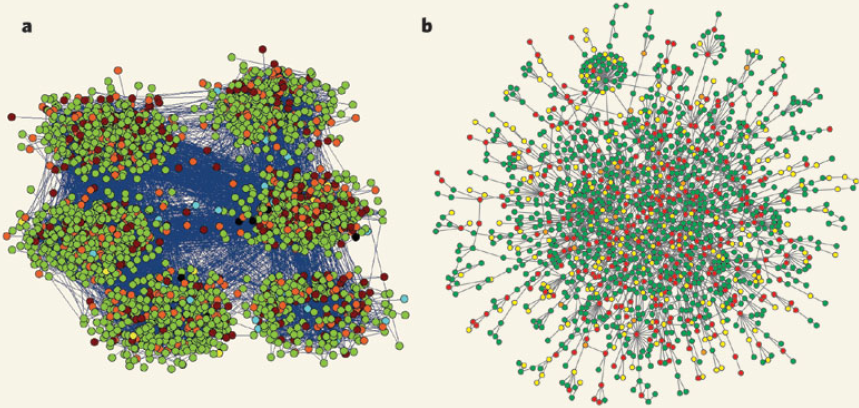
\includegraphics[height=6cm]{assort_disassort}

a: school communities; 

b: proteins in brewer's yeast.
\end{frame}

\subsection{Stupid Ideas}
\begin{frame}
\frametitle{Concepts}
\begin{itemize}
\item Clique, complete subgraphs.
\item Density $\frac{\text{avg deg}}{\text{complete deg}}$
\item Modularity: the extent of module-divided formation of networks.
Defined as: measurement of extra edges aside of random connection.
\end{itemize}
\end{frame}



\section{Algorithms}
\begin{frame}
\frametitle{Algorithms}
\begin{itemize}
\item Heirachical
\item Information theory
\item Graph theory
\item Other stupid fantacies
\end{itemize}
\end{frame}

\begin{frame}
\frametitle{Erdos-Renyi probability based graph model.}
Erdos-Renyi probability based graph model.1959

\begin{itemize}
\item $Pr(m)=\binom{\binom{n}{2}}{m} p^m (1-p)^{\binom{n}{2}-m}$
\item $\mathbb{E}[m]=\binom{n}{2}p,\mathbb{E}[k]=\frac{2}{n}\binom{n}{2}p$
\item $Pr(k)=\binom{n-1}{k}p^k(1-p)^{(n-1-k)}$

$Pr(k)\simeq \frac{c^k}{k!}e^c$ (Poisson)
\end{itemize}
\end{frame}


\begin{frame}
\frametitle{Erdos-Renyi probability based graph model.}
Phase Transition
\begin{itemize}
\item $Pr(\neg e_{i,j})=1-p$,$Pr(e_{i,j} \land \neg e_{j,compo})=pu$
\item $u=(1-p+pu)^{n-1}=[1-\frac{c(1-u)}{n-1}]^{n-1}$
\item $\lim_{n \rightarrow \infty} u = e^{-c(1-u)}$, $Pr(e_{i,comp})=1-u=S$
\item $\lim_{n \rightarrow \infty} S = 1-e^{-cS}$
\end{itemize}
\end{frame}

\begin{frame}
\frametitle{Erdos-Renyi probability based graph model.}
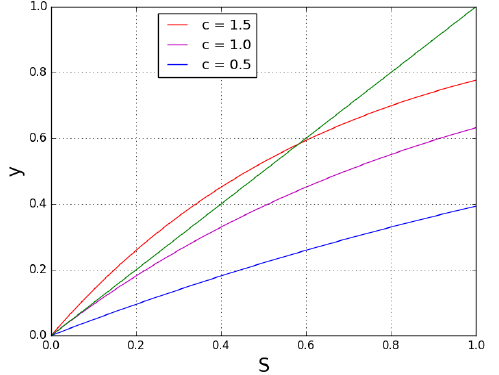
\includegraphics[height=6cm]{s_prob}

$S = 1-e^{-cS}$,if, $S>\frac{\ln(c)}{c}$,  $c\geq 1$
\end{frame}


\begin{frame}
\frametitle{Girvan - Newman algorithm}
Girvan - Newman algorithm 2004

Sometimes wrongly called NG.

Some preceding concepts:
\begin{itemize}
\item Vertex bewteeneess
\item Edge betweenness
\item Pareto principle: 80/20 rule
\end{itemize}
\end{frame}


\begin{frame}
\frametitle{Girvan - Newman algorithm}
Fundamental ideas:
\begin{itemize}
\item Power-law/Pareto principle yield isolation 
\item The minorities act as gate-nodes
\item Removing those path reveals the communities.
\end{itemize}
\end{frame}


\begin{frame}
\frametitle{Girvan - Newman algorithm}
Dendrogram Breadth first
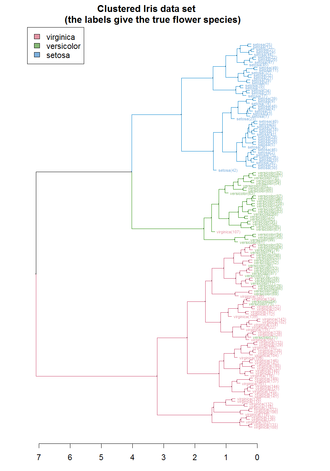
\includegraphics[height=8cm]{dendrogram}
\end{frame}


\begin{frame}
\frametitle{Latent Semantic Analysis}
Latent Semantic Analysis 1988
\begin{eqnarray}
D=\{d_1,d_2,..,d_{N} \} \\
W=\{w_1,w_2,..,w_{M} \} \\
Z=\{ z_1,z_2,..,z_{K} \} \\
A_{coappearance} \text{ is }  N \times M \\
A=U_{N \times r } \Sigma_{r \times r} V^{T}_{r \times M } \text{ (SVD/NMF) }
\end{eqnarray}
\end{frame}


\begin{frame}
\frametitle{Probablistic Latent Semantic Analysis}
Probablistic Latent Semantic Analysis 2000,

by Thomas Hofmann.
\begin{eqnarray}
P(d_i,w_j)& =& P(d_i) P(w_j | d_i), \\
P(w_j | d_i) &=& \sum_{k=1}^{K} P(w_j | z_k) P(z_k | d_i) \\
\mathcal{L} &=& \sum_{i=1}^N \sum_{j=1}^M n(d_i,w_j) \log P(d_i,w_i)
\end{eqnarray}
\end{frame}


\begin{frame}
\frametitle{Probablistic Latent Semantic Analysis}
\begin{eqnarray}
{\color{red} P(z_k|d_i,w_j) } = \frac{P(z_k)P(d_i|z_k)P(w_j|z_k)}{P(d_i,w_j)} \\
\text{E}[\mathcal{L}] =  \sum_{i=1}^N \sum_{j=1}^M n(d_i,w_j) \sum_{k=1}^{K} \cdot \cdot \cdot  \\
{\color{red} P(z_k|d_i,w_j) } \log  P(w_j|z_k)P(z_k|d_i)
\end{eqnarray}
\end{frame}


\begin{frame}
\frametitle{Probablistic Latent Semantic Analysis}
Expectation Maximization
\begin{eqnarray}
\sum_{j} P(w_j|z_k) =1\\
\sum_{i} P(z_k|d_i) =1\\
KKT:\frac{\partial L }{\partial {\color{red} P(w_j|z_k) }} =0, \frac{\partial L}{\partial {\color{red} P(z_k|d_i)} } =0
\end{eqnarray}
MASHA, HPLSA, Latent Dirichlet allocation
\end{frame}

\begin{frame}
\frametitle{Dual problem}
Dual problem
\begin{itemize}
\item $f(x), s.t. g(x) \le 0$
\item $L(x,\lambda) = f(x) + \lambda g(x), \lambda \geq 0$
\item $argmax_\lambda L = f =$ initial problem
\item we define original problem as :

$argmin_x argmax_\lambda L(x,\lambda) s.t. \lambda \geq 0, g(x) \leq 0$

\item $ L(x^*,\lambda) \leq L(x^*,\lambda^*)  \leq L(x,\lambda^*)$
\item Karush-Kuhn-Tucker conditions
\end{itemize}
\end{frame}

\begin{frame}
\frametitle{Dual problem}
Dual problem-KKT conditions
\begin{itemize}
\item $\lambda^* g(x^*)=0$
\item $\frac{\partial L}{  \partial x} =0$ 
\item $\lambda \geq 0 , g(x) \leq 0$
\end{itemize}
KKT is necessary and sufficient condition.
\begin{itemize}
\item $\max_\lambda \min_x L(x,\lambda) , s.t. \lambda \geq 0, g(x) \leq 0$
\item KKT $\rightarrow x=h(\lambda)$
\item $\max_\lambda L(h(\lambda),\lambda) s.t. \lambda \geq 0, S(\lambda)=0$
\end{itemize}
\end{frame}

\begin{frame}
\frametitle{Expectation Maximization}
Expectation Maximization
\begin{itemize}
\item $f(x;\theta) \rightarrow f(x,y;\theta)$
\item randomize $\theta, y$
\item estimate $Q=q(y,\theta)$ (E-step)
\item $\frac{\partial -L(Q)}{\partial \theta}=0$,update $\theta$ (M-step)
\item repeat until converge.
\end{itemize}
\end{frame}


\begin{frame}
\frametitle{Expectation Maximization}
\begin{itemize}
\item Jensen's inequality $f(\sum \lambda x) \leq \sum \lambda f(x)$
\item $\sum \log \sum p \geq \sum \sum Q \log \frac{p}{Q}=l(\theta) $
\item $l(\theta)$ is the lower bound. 
\item $f(E_z[\frac{p(x,z;\theta)}{Q(z)}]) \geq E_z[f(\frac{p(x,z;\theta)}{Q(z)})]$
\item $\frac{p}{Q}=Const$ s.t. $\sum_z Q(z)=1$
\item $Q(z)=\frac{p(x,z)}{\sum p(x)}=p(z|x;\theta)$
\end{itemize}
\end{frame}

\begin{frame}
\frametitle{Ball,Karrer,Newman algorithm}
Brian Ball, Brian Karrer, M. E. J. Newman 2011
\begin{itemize}
\item generative model
\item use Z colors to annotate communities
\item vertex $v_i$ has Z params $\theta_{iz}$
\item $P(Edge(v_i,v_j)) = \sum_{z} \theta_{iz} \theta_{jz}$
\item EM for $\theta$
\end{itemize}
\end{frame}

\begin{frame}
\frametitle{Ball,Karrer,Newman algorithm}
BKN is able to detect overlappings.

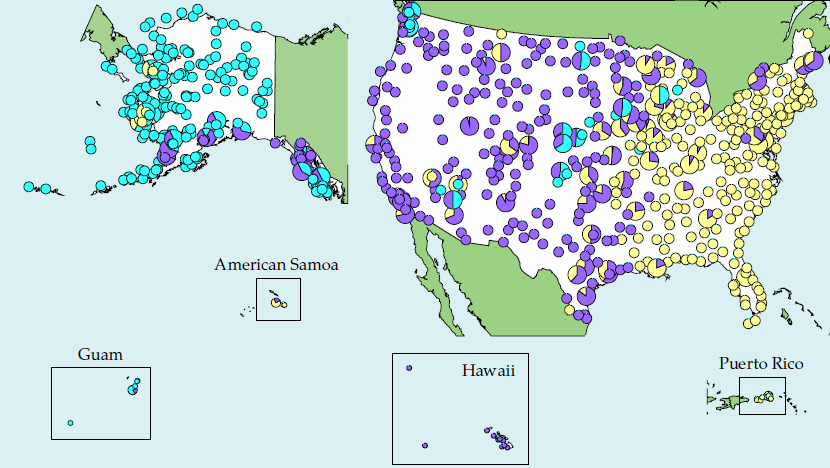
\includegraphics[height=6cm]{bkn}
\end{frame}


\begin{frame}
\frametitle{Latent community discovery network}
Latent community discovery network 2012 (Tsinghua). (PLSA-like)
\begin{itemize}
\item users with significant influence: core actors $a_i$.
\item ordinary user $u$
\item document of u, $d=a_1,...,a_{|d|}$, network $n$ 
\item \textbf{c}ount(a,d): occurrence of a in d.
\item topics $z$
\end{itemize}
\end{frame}


\begin{frame}
\frametitle{Latent community discovery network}
\begin{itemize}
\item how to get a list of core actors?
\item $\sum_z P(z|d)=1$,(mixing) 
\item $\sum_a P(a|z)=1$ (topics are prevailing)
\item $L=\sum_d \sum_a C(a,d) \log \sum_z P(a|z)P(z|d)$
\item $R=\sum_{a1,a2} \sum_z \|p(z|a_1) - p(z|a_2)\|^2$ what?
\end{itemize}
\end{frame}


\begin{frame}
\frametitle{Latent community discovery network}
\begin{itemize}
\item $Objective=\alpha (-L) + (1-\alpha)R$
\item EM again.
\end{itemize}
\end{frame}

\begin{frame}
\frametitle{Latent community discovery network}
AI DB DP GV NC

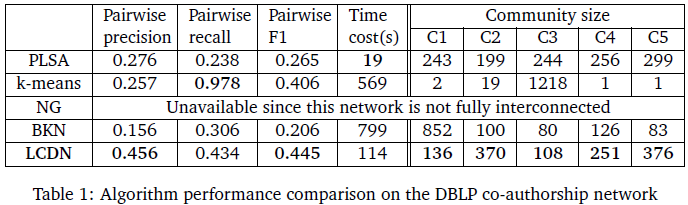
\includegraphics[height=3.5cm]{lcdndblp}

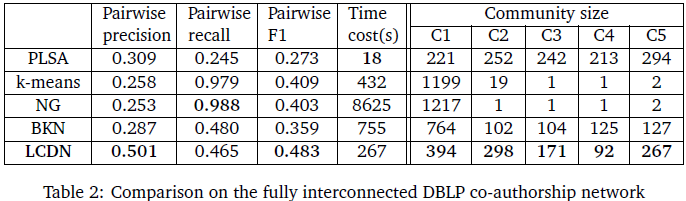
\includegraphics[height=3.5cm]{lcdndblpfully}
\end{frame}

\begin{frame}
\frametitle{Latent community discovery network}
1. Entertainment244 2. Leisure,  333 

3. Finance,  297 4. Culture,  185

5. Media,  163 
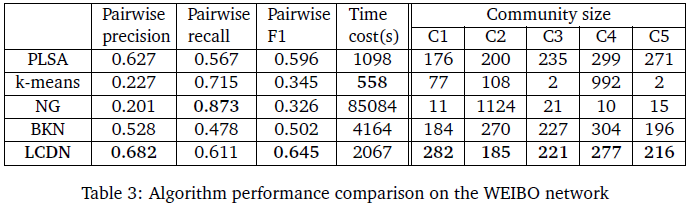
\includegraphics[height=3.5cm]{lcdnweibo}

If you torture the data long enough, data will confess.
\end{frame}



\begin{frame}
\frametitle{Page rank}
Page rank 1998.
\begin{itemize}
\item incoming-links: other $\rightarrow$ this site.
\item Pagerank(site) $PR(site)$
\item $PR(A)=\left( \frac{PR(B)}{L(B)} + \frac{PR(C)}{L(C)} + \cdots \right)d + \frac{1-d}{N}$
\item $(1-d)$
\end{itemize}
\end{frame}

\begin{frame}
\frametitle{Page rank Ideal rank Approxrank}
\begin{itemize}
\item Idealrank 2009: local pagerank. far-away PR-values are simplified and unified.
\item $\lim_{\substack{edge \rightarrow full \\ V_{local} \rightarrow V_{global} } } Idealrank= Pagerank$
\item approxrank 2009:  $approxrank \sim Idealrank$
\end{itemize}
\end{frame}

\begin{frame}
\frametitle{Trust Network}
Trust Network
\begin{itemize}
\item e-commerce
\item resource sharing
\item SQA,SDN
\item propagenda
\item promotion/ads
\end{itemize}
\end{frame}

\begin{frame}
\frametitle{Trust Network}
Zhang shaozhong. et al.  2012
\begin{itemize}
\item Interactions matrix $A$
\item Successful Interactions matrix $T$
\item Faliures $F$
\item $Believe(v_i,v_j)=\sum \sum p(v_i,v_j) \log \frac{p(v_i,v_j)}{p(v_i)p(v_j)} $
\item $v$: success or failure.
\end{itemize}
\end{frame}


\begin{frame}
\frametitle{Trust Network}
Mutual information

$I(X;Y) = \sum_y \sum_x  p(x,y) \log \frac{p(x,y)}{p(x)p(y)} $

if $X, Y$, iid. then $ I=0$

else $ I > 0 $
\end{frame}

\begin{frame}
\frametitle{Trust Network}
To find an optimal trusty path:
\begin{itemize}
\item Floyd
\item Dijkstra
\end{itemize}
How to find communities?
\end{frame}

\begin{frame}
\frametitle{Trust Network}
How to find communities?
\begin{itemize}
\item interconnectivity in v $C_v = \frac{2t_v}{k_v(k_v-1)} $
\item $\text{E}[C_v]=C=\frac{\sum_{n=1}^{\infty} C_v}{n} $
\item characteristic path length: $\frac{\sum_i \frac{\sum_j MinDist(i,j)}{n-1}  }{n} $
\end{itemize}
\end{frame}


\begin{frame}
\frametitle{Trust Network}
How to find communities?
\begin{itemize}
\item $ f = a \left( \sum Believe \right) + b C|_m $
\item cut $m$ weak interactions. (heirachical?)
\item {\color{red} NP hard!}
\item a heuristic algorithm:
 \item [1] cut $m$ edges $e_1,..,e_m$ that maximize $f$.
 \item [2]  add $e_m'$ that maximize $f$, if $e_m' =e_m$ over.
 \item [3] cut one edge that maximize $f$, then go to 2.
\end{itemize}
\end{frame}


\begin{frame}
\frametitle{End}
\Huge Thank you, gays.
\end{frame}


\begin{frame}
\frametitle{}
\begin{itemize}
\item a
\item b
\end{itemize}
\end{frame}


%============================================================
%============================================================
%============================================================
%============================================================
%============================================================
%============================================================

\begin{frame}
\frametitle{Paragraphs of Text}
Sed iaculis dapibus gravida. Morbi sed tortor erat, nec interdum arcu. Sed id lorem lectus. Quisque viverra augue id sem ornare non aliquam nibh tristique. Aenean in ligula nisl. Nulla sed tellus ipsum. Donec vestibulum ligula non lorem vulputate fermentum accumsan neque mollis.\\~\\

Sed diam enim, sagittis nec condimentum sit amet, ullamcorper sit amet libero. Aliquam vel dui orci, a porta odio. Nullam id suscipit ipsum. Aenean lobortis commodo sem, ut commodo leo gravida vitae. Pellentesque vehicula ante iaculis arcu pretium rutrum eget sit amet purus. Integer ornare nulla quis neque ultrices lobortis. Vestibulum ultrices tincidunt libero, quis commodo erat ullamcorper id.
\end{frame}

%------------------------------------------------

\begin{frame}
\frametitle{Bullet Points}
\begin{itemize}
\item Lorem ipsum dolor sit amet, consectetur adipiscing elit
\item Aliquam blandit faucibus nisi, sit amet dapibus enim tempus eu
\item Nulla commodo, erat quis gravida posuere, elit lacus lobortis est, quis porttitor odio mauris at libero
\item Nam cursus est eget velit posuere pellentesque
\item Vestibulum faucibus velit a augue condimentum quis convallis nulla gravida
\end{itemize}
\end{frame}

%------------------------------------------------

\begin{frame}
\frametitle{Blocks of Highlighted Text}
\begin{block}{Block 1}
Lorem ipsum dolor sit amet, consectetur adipiscing elit. Integer lectus nisl, ultricies in feugiat rutrum, porttitor sit amet augue. Aliquam ut tortor mauris. Sed volutpat ante purus, quis accumsan dolor.
\end{block}

\begin{block}{Block 2}
Pellentesque sed tellus purus. Class aptent taciti sociosqu ad litora torquent per conubia nostra, per inceptos himenaeos. Vestibulum quis magna at risus dictum tempor eu vitae velit.
\end{block}

\begin{block}{Block 3}
Suspendisse tincidunt sagittis gravida. Curabitur condimentum, enim sed venenatis rutrum, ipsum neque consectetur orci, sed blandit justo nisi ac lacus.
\end{block}
\end{frame}

%------------------------------------------------

\begin{frame}
\frametitle{Multiple Columns}
\begin{columns}[c] % The "c" option specifies centered vertical alignment while the "t" option is used for top vertical alignment

\column{.45\textwidth} % Left column and width
\textbf{Heading}
\begin{enumerate}
\item Statement
\item Explanation
\item Example
\end{enumerate}

\column{.5\textwidth} % Right column and width
Lorem ipsum dolor sit amet, consectetur adipiscing elit. Integer lectus nisl, ultricies in feugiat rutrum, porttitor sit amet augue. Aliquam ut tortor mauris. Sed volutpat ante purus, quis accumsan dolor.

\end{columns}
\end{frame}

\begin{frame}
\frametitle{Table}
\begin{table}
\begin{tabular}{l l l}
\toprule
\textbf{Treatments} & \textbf{Response 1} & \textbf{Response 2}\\
\midrule
Treatment 1 & 0.0003262 & 0.562 \\
Treatment 2 & 0.0015681 & 0.910 \\
Treatment 3 & 0.0009271 & 0.296 \\
\bottomrule
\end{tabular}
\caption{Table caption}
\end{table}
\end{frame}

%------------------------------------------------

\begin{frame}
\frametitle{Theorem}
\begin{theorem}[Mass--energy equivalence]
$E = mc^2$
\end{theorem}
\end{frame}

%------------------------------------------------

\begin{frame}[fragile] % Need to use the fragile option when verbatim is used in the slide
\frametitle{Verbatim}
\begin{example}[Theorem Slide Code]
\begin{verbatim}
\begin{frame}
\frametitle{Theorem}
\begin{theorem}[Mass--energy equivalence]
$E = mc^2$
\end{theorem}
\end{frame}\end{verbatim}
\end{example}
\end{frame}

%------------------------------------------------

\begin{frame}
\frametitle{Figure}
Uncomment the code on this slide to include your own image from the same directory as the template .TeX file.
%\begin{figure}
%\includegraphics[width=0.8\linewidth]{test}
%\end{figure}
\end{frame}

%------------------------------------------------

\begin{frame}[fragile] % Need to use the fragile option when verbatim is used in the slide
\frametitle{Citation}
An example of the \verb|\cite| command to cite within the presentation:\\~

This statement requires citation \cite{p1}.
\end{frame}

%------------------------------------------------

\begin{frame}
\frametitle{References}
\footnotesize{
\begin{thebibliography}{99} % Beamer does not support BibTeX so references must be inserted manually as below
\bibitem[Smith, 2012]{p1} John Smith (2012)
\newblock Title of the publication
\newblock \emph{Journal Name} 12(3), 45 -- 678.
\end{thebibliography}
}
\end{frame}

%------------------------------------------------

\begin{frame}
\Huge{\centerline{The End}}
\end{frame}

%----------------------------------------------------------------------------------------

\end{document} 